\documentclass[conference]{IEEEtran}
\usepackage[utf8]{inputenc}
\usepackage[T1]{fontenc}
\usepackage{amsmath,amssymb}
\usepackage{graphicx}
\usepackage{booktabs}
\usepackage{array}
\usepackage{url}
\usepackage[hidelinks]{hyperref}
\usepackage[ruled,vlined,linesnumbered]{algorithm2e}
\graphicspath{{../figures/}}
\SetKwInput{KwInput}{Input}
\SetKwInput{KwOutput}{Output}

\title{Ensemble Methods: Boosting vs. Bagging}

\author{
\IEEEauthorblockN{Shahin Safarli, Gulnisa Abdurahmanli, Jeyhuna Sevdiyeva, Seljan Khasiyeva, Suleyman Allahverdiyev}
\IEEEauthorblockA{AI Academy, National AI Center\\
Machine Learning, Spring 2026}
}

\begin{document}
\maketitle

\begin{abstract}
This paper studies when boosting and bagging are preferable by implementing
Decision Trees, AdaBoost, Random Forests, PCA, K-Means, DBSCAN, and a bonus
Gradient Boosting classifier from scratch. The locked study uses all 569
Breast Cancer rows, all 48,842 Adult rows, an exact seed-42 seven-class sample
of 50,000 Covertype rows, and all 14,780 MNIST zeros and ones. Every supervised
fold fits mixed-type preprocessing and any imbalance treatment on training
rows only. We compare accuracy, macro F1, macro/binary AUC, scaling, label
noise, and a 100-bootstrap Breast Cancer bias-variance decomposition. Complete
transformed arrays also feed PCA, K-Means, and exact KD-tree DBSCAN, while the
t-SNE bonus uses every MNIST2Class row. The resulting evidence distinguishes
sequential bias correction from parallel variance reduction across medical,
mixed tabular, multiclass imbalanced, and high-dimensional image settings.
\end{abstract}

\section{Introduction}
\IEEEPARstart{B}{oosting} and bagging both combine decision-tree learners, but
they attack different failure modes. Boosting is sequential: each weak learner
is trained on a distribution that emphasizes examples misclassified by the
previous ensemble. Bagging is parallel: it trains high-variance predictors on
bootstrap samples and averages their outputs to reduce variance. The central
question is therefore empirical and conditional: under what data conditions
does one ensemble philosophy outperform the other, and why?

We answer this question with from-scratch implementations rather than
wrapping sklearn ensemble classes. The supervised code includes a weighted
CART-style decision tree, a depth-1 decision stump, SAMME AdaBoost, and
Random Forest with bootstrap sampling, feature subsampling, out-of-bag (OOB)
evaluation, and hard majority voting. The unsupervised code includes PCA,
K-Means, and DBSCAN. Sklearn is used only for dataset loading, metrics,
cross-validation utilities, t-SNE, and explicitly marked reference baselines.
Every experiment is reproducible with
\texttt{python src/experiments/run\_all.py}. First-run downloads are cached
only in ignored raw/sklearn/interim directories; \texttt{--skip-downloads}
requires those authoritative caches and fails if any required data are absent.

The contribution of the study is not only a ranking of algorithms. We connect
observed performance to heterogeneous features, high dimensionality, label
noise, and multiclass imbalance. This matters because accuracy alone can be
misleading when common Covertype classes dominate rare classes.
For that reason we report accuracy, macro F1, and AUC-ROC, and we interpret
the metrics jointly.

\section{Related Work}
Decision trees recursively partition feature space using impurity reduction.
We follow CART-style binary splits with Gini impurity or entropy
\cite{hastie2009elements,quinlan1986induction}. For a node with weighted
class counts $n_c$, the Gini impurity is
$1-\sum_c (n_c/\sum_j n_j)^2$, while entropy is
$-\sum_c p_c\log_2 p_c$. A split is accepted only when it produces a positive
weighted impurity reduction, matching the project rule that a node becomes a
leaf if no split reduces impurity.

AdaBoost constructs an additive classifier by increasing the weights of
misclassified observations and assigning each weak learner a coefficient
based on its weighted error \cite{freund1997decision}. Bagging reduces
variance by averaging predictors trained on bootstrap samples
\cite{breiman1996bagging}. Random Forests add feature subsampling at each
split to decorrelate trees further \cite{breiman2001random}. PCA, K-Means,
and DBSCAN are used to inspect the geometry of each dataset before
classification \cite{pearson1901lines,lloyd1982least,ester1996density}. The
bonus t-SNE visualization follows van der Maaten and Hinton
\cite{maaten2008visualizing}; the bonus Gradient Boosting comparison follows
Friedman's additive modeling view \cite{friedman2001greedy}.

\section{Methods}
\subsection{Decision Tree and Stump}
The tree stores at every node the split feature, threshold, child pointers,
weighted class distribution, sample count, impurity, and weighted impurity
decrease. Continuous thresholds are midpoints between adjacent sorted feature
values. During fitting, each feature is sorted once per node and candidate
left/right class counts are accumulated with vectorized cumulative sums.
This makes weighted split evaluation efficient enough for the ensemble
experiments while remaining transparent for defense.

Stopping conditions are: maximum depth reached, fewer than
\texttt{min\_samples\_split} samples, pure node, identical feature vectors, or
no positive impurity-improving split. Weighted class counts are used for both
Gini/entropy and predicted leaf probabilities. The same code path supports
AdaBoost because \texttt{fit} accepts \texttt{sample\_weight}. Feature
importance is computed as the normalized sum of weighted impurity decreases
over internal nodes. The \texttt{DecisionStump} is a depth-1 specialization
with the same weighted impurity logic.

\subsection{AdaBoost}
The required AdaBoost implementation uses decision stumps as weak learners.
At round $m$, a weighted stump $h_m$ is fit, its weighted error
$\epsilon_m$ is measured, and the sample weights are updated by
\[
w_i^{(m+1)} \propto w_i^{(m)}
\exp(\alpha_m \mathbf{1}[h_m(x_i)\ne y_i]).
\]
For multiclass SAMME,
\[
\alpha_m=\eta\left(\log\frac{1-\epsilon_m}{\epsilon_m}+
\log(K-1)\right),
\]
where $K$ is the number of classes and $\eta$ is the learning rate. The
implementation also includes a bonus SAMME.R path that accumulates centered
log-probability scores from the stump probabilities. Staged predictions are
stored so the scaling experiment can plot training and test error from 1 to
200 boosting rounds without refitting. Algorithm~\ref{alg:adaboost} states the
full training loop implemented by \texttt{AdaBoostClassifier.fit}, matching
the interface contract required by the project brief.

\begin{algorithm}[t]
\SetAlgoLined
\KwInput{Training data $(x_i,y_i)_{i=1}^n$, rounds $M$, learning rate $\eta$}
\KwOutput{Weighted ensemble of stumps $\{(h_m,\alpha_m)\}_{m=1}^M$}
Initialize weights $w_i^{(1)} = 1/n$ for all $i$\;
\For{$m \gets 1$ \KwTo $M$}{
  Fit stump $h_m$ on weighted data $(x_i, y_i, w_i^{(m)})$\;
  $\epsilon_m \gets \sum_i w_i^{(m)} \mathbf{1}[h_m(x_i)\ne y_i] \big/ \sum_i w_i^{(m)}$\;
  \If{$\epsilon_m \ge 1 - 1/K$}{
    stop early (weak learner no better than chance)\;
  }
  $\alpha_m \gets \eta\left(\log\frac{1-\epsilon_m}{\epsilon_m} + \log(K-1)\right)$\;
  $w_i^{(m+1)} \gets w_i^{(m)} \exp(\alpha_m \mathbf{1}[h_m(x_i)\ne y_i])$ for all $i$\;
  Renormalize $w^{(m+1)}$ to sum to 1\;
}
Store staged predictions using cumulative weighted votes of $h_1,\dots,h_m$ for every $m$\;
\caption{SAMME AdaBoost training, as implemented by \texttt{AdaBoostClassifier.fit}.}
\label{alg:adaboost}
\end{algorithm}

The per-round cost is dominated by fitting a stump, which is
$O(nd\log n)$ for $n$ weighted samples and $d$ features because every
feature is sorted once and candidate thresholds are scanned with a single
cumulative pass. Training the full ensemble is therefore
$O(Mnd\log n)$, linear in the number of rounds $M$. Because a stump has
exactly one split, AdaBoost's capacity grows by adding more weak
learners rather than by deepening any single learner, which is why the
scaling experiment (Fig.~\ref{fig:boosting}) plots error against $M$ rather
than tree depth.

\subsection{Random Forest}
Each Random Forest tree is trained on a bootstrap sample of the training set.
The implementation records OOB indices for every tree, samples
\texttt{sqrt} candidate features by default at each split, and stores per-tree
seeds for deterministic reproduction. The \texttt{predict} method follows the
project brief exactly: it uses hard majority vote across trees. Probability
prediction is still provided by averaging aligned per-tree leaf
probabilities, which is useful for AUC. Alignment is necessary on the
seven-class Covertype setting because a bootstrap sample can omit a small class; in
that case a tree's probability columns must be mapped back to the forest's
global class order.

\begin{algorithm}[t]
\SetAlgoLined
\KwInput{Training data $(x_i,y_i)_{i=1}^n$, forest size $T$, feature
subsample size $m\!\approx\!\sqrt{d}$}
\KwOutput{Trees $\{f_t\}_{t=1}^T$ with recorded OOB index sets}
\For{$t \gets 1$ \KwTo $T$}{
  Draw bootstrap sample $B_t$ of size $n$ with replacement from $\{1,\dots,n\}$\;
  Record OOB indices $O_t \gets \{1,\dots,n\}\setminus B_t$\;
  Fit full-depth tree $f_t$ on $B_t$, restricting every split search to a
  fresh random subset of $m$ features\;
}
\textbf{Predict:} $\hat{y}(x) = \operatorname{mode}\{f_1(x),\dots,f_T(x)\}$
(hard majority vote)\;
\textbf{OOB score:} for each $i$, aggregate votes only from trees where
$i \in O_t$, then average agreement with $y_i$\;
\caption{Bagging with feature subsampling, as implemented by
\texttt{RandomForestClassifier.fit}.}
\label{alg:rf}
\end{algorithm}

Because every tree in Algorithm~\ref{alg:rf} is grown on an independent
bootstrap sample, the trees are only weakly correlated; feature subsampling
at each split decorrelates them further, which is the mechanism Breiman
identifies as reducing forest variance below single-tree variance
\cite{breiman2001random}. Fitting $T$ full-depth trees costs
$O(Tnd\log^2 n)$ in the worst case (depth $O(\log n)$ times the per-level
$O(nd)$ split search), so Random Forest is more expensive per estimator
than AdaBoost's stumps, but the trees can be fit independently, which is why
the implementation supports optional \texttt{n\_jobs} multiprocessing while
AdaBoost's sequential dependency prevents that same parallelization.

\subsection{Unsupervised Pipeline and Bonuses}
PCA is implemented by covariance eigen-decomposition after centering. K-Means
uses k-means++ initialization, Lloyd updates, inertia tracking, and repeated
restarts. DBSCAN uses a private balanced exact KD-tree with bounding-box
pruning. Radius neighborhoods are queried lazily during cluster expansion,
and the same index answers exact $k$-nearest queries for the sorted fifth-
nonself-neighbor curve. No $n\times n$ distance matrix or complete
neighborhood list is retained; labels remain deterministic and noise is $-1$.
The unsupervised pipeline serves two purposes. First, it verifies that the
project can analyze data geometry without labels. Second, it gives context
for classification: when PCA clusters align with labels, simpler tree splits
and stumps are more likely to work; when alignment is weak, bagging over full
trees tends to be safer. Bonus work includes t-SNE figures, multiclass
SAMME.R support, a binary Gradient Boosting classifier with logistic loss,
GitHub Actions CI, and an interactive notebook.

Cluster fitting itself never receives class labels, but configuration reporting
is explicitly label-informed: the runner evaluates K-Means for $k=1,\ldots,10$
and reports the solution with the highest ARI, while DBSCAN evaluates exact
fifth-neighbor-distance percentile candidates and reports the best
$\mathrm{ARI}-0.05\times\mathrm{noise\ fraction}$ trade-off. The elbow and
$k$-distance plots are descriptive diagnostics. Consequently, the clustering
results are exploratory comparisons against known labels, not evidence of a
fully unsupervised model-selection procedure.

\section{Experimental Setup}
Table~\ref{tab:datasets} summarizes the locked four-dataset contract
\cite{uciAdult,uciCovertype,openmlMnist}. Breast
Cancer uses all packaged rows. Adult combines the 32,561 official training
and 16,281 test records without dropping missing values. After indices are
split, numeric median imputation and scaling and categorical mode imputation
and one-hot categories are fit on the training rows only; unseen held-out
categories map to all-zero indicator groups. Covertype remains seven-class
and uses a seed-42 exact largest-remainder stratified selection of 50,000 from
all 581,012 rows. MNIST2Class retains every zero and one in OpenML
\texttt{mnist\_784} v1. For Covertype, each underrepresented class is randomly
oversampled only inside the training fold toward 25\% of the majority count,
identically for every compared model.

\begin{table}[t]
\centering
\caption{Datasets used in the study.}
\label{tab:datasets}
\begin{tabular}{lccc}
\toprule
Dataset & Samples & Raw features & Classes \\
\midrule
Breast Cancer Wisconsin & 569 & 30 & 2 \\
Adult Income & 48,842 & 14 mixed & 2 \\
Covertype & 50,000 & 54 & 7 \\
MNIST2Class & 14,780 & 784 & 2 \\
\bottomrule
\end{tabular}
\end{table}

All random seeds are fixed at 42 unless a fold or replicate offset is needed.
The seven required experiments are: baseline trees, AdaBoost scaling,
Random Forest scaling, 5-fold head-to-head comparison, label-noise
robustness, bias-variance decomposition with 100 bootstraps, and
unsupervised analysis. Binary AUC uses the positive-class probability.
Multiclass AUC uses one-vs-rest macro averaging. Bias-variance uses the real
stratified 80/20 Breast Cancer split, 100 bootstrap resamples of its fixed
training partition, and predictions on the unchanged clean test partition.

\subsection{Hyperparameter and Design Choices}
Every supervised hyperparameter used in the experiments is fixed in advance
rather than tuned on test folds, so the reported predictive numbers are not
the result of implicit test-set leakage. The separate clustering analysis uses
the explicitly disclosed post-hoc ARI criteria described above. AdaBoost uses
learning rate $\eta=0.6$: values
close to 1 let a single very confident stump dominate early rounds, while
smaller values shrink each stump's contribution and rely on more rounds to
reach the same training error, trading round-count for stability. We chose
$0.6$ because it is small enough to keep the SAMME weight update numerically
well behaved across the binary and seven-class tasks while still using the
200-round budget effectively.
Random Forest uses $\texttt{max\_features="sqrt"}$, the classical
decorrelation choice from \cite{breiman2001random}: smaller subsets
decorrelate trees more but each split search sees less signal, and $\sqrt{d}$
is the standard compromise recommended for classification forests. The
imbalance oversampling ratio of 25\% was chosen so that rare Covertype classes
are exposed to every learner without duplicating them to a perfectly balanced
1:1 target, which would misrepresent inference-time prevalence. All values are
constants declared once at the top of \texttt{src/experiments/run\_all.py}
and reused by every experiment, so there are no hard-coded magic numbers
scattered through the codebase.

\section{Results}
\subsection{Baseline Sanity Check}
Table~\ref{tab:baseline} isolates the custom tree before ensemble effects.
The largest absolute accuracy gap to an entropy-matched sklearn reference is
0.018 on Breast Cancer; all four gaps remain within the required two
percentage points. Covertype also demonstrates why one stump is not an
adequate multiclass learner: its accuracy is 0.436 versus 0.811 for the full
custom tree.

\begin{table}[t]
\centering
\caption{Baseline test accuracy. Gap is the absolute difference between the
custom and sklearn trees.}
\label{tab:baseline}
\begin{tabular}{lcccc}
\toprule
Dataset & Tree & Stump & sklearn & Gap \\
\midrule
Breast Cancer & 0.956 & 0.823 & 0.938 & 0.018 \\
Adult Income & 0.821 & 0.761 & 0.817 & 0.004 \\
Covertype & 0.811 & 0.436 & 0.810 & 0.001 \\
MNIST2Class & 0.996 & 0.986 & 0.995 & 0.001 \\
\bottomrule
\end{tabular}
\end{table}

\subsection{Scaling Behavior}
Figure~\ref{fig:boosting} shows all 21 AdaBoost checkpoints. At 200 rounds,
test error is 0.035 on Breast Cancer, 0.141 on Adult, 0.403 on Covertype,
and 0.001 on MNIST2Class. Breast Cancer and MNIST2Class reach zero training
error, whereas the seven-class Covertype task remains difficult for a
sequence of axis-aligned stumps even after training-fold oversampling.

\begin{figure}[t]
\centering
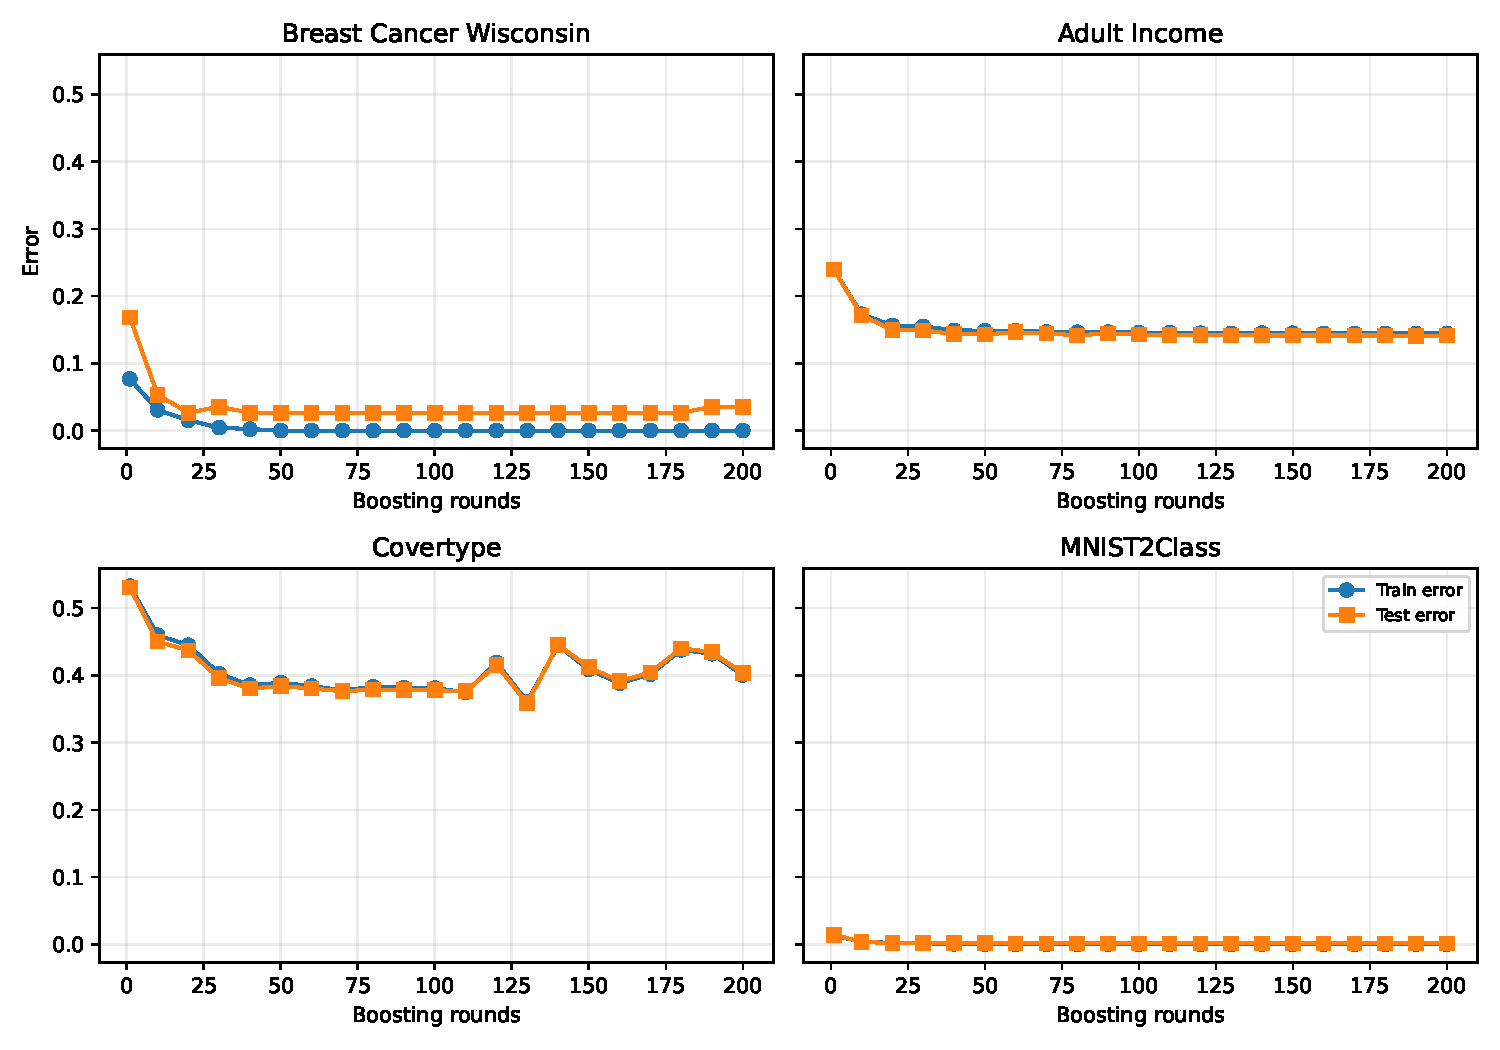
\includegraphics[width=\linewidth]{adaboost_scaling.pdf}
\caption{AdaBoost train and test error on the four required datasets.}
\label{fig:boosting}
\end{figure}

Random Forest test accuracy at 200 trees is 0.965, 0.868, 0.816, and 0.999
in the same dataset order; the corresponding OOB values are 0.956, 0.864,
0.871, and 0.998. The Covertype OOB value is evaluated on the transformed,
oversampled training distribution, so its difference from the untouched test
distribution is expected and it must not be read as a held-out replacement.
Figures~\ref{fig:rf} and~\ref{fig:rfdepth} show that estimator count and
depth stabilize at dataset-specific rates.

\begin{figure}[t]
\centering
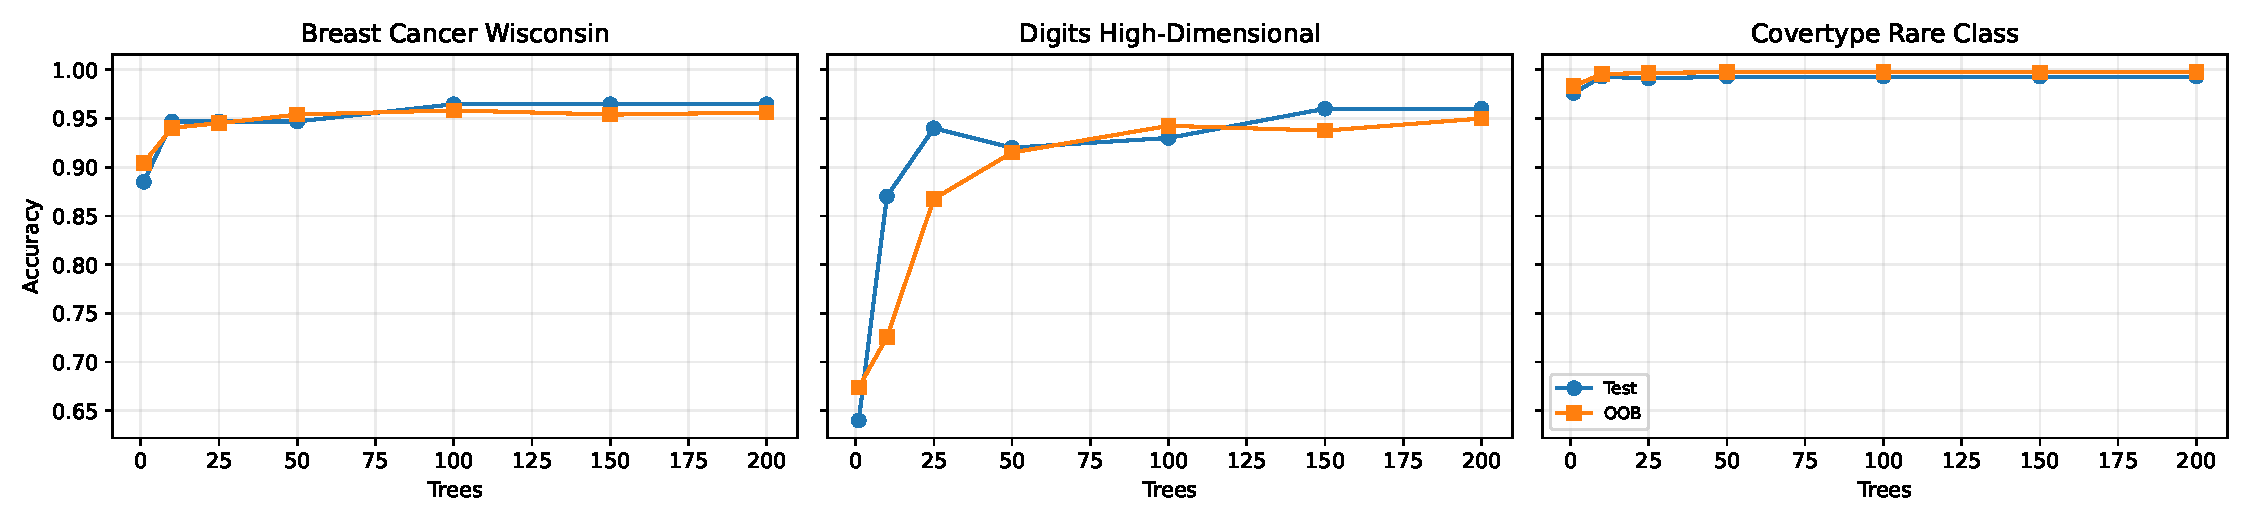
\includegraphics[width=\linewidth]{random_forest_estimators.pdf}
\caption{Random Forest test and OOB accuracy versus estimator count.}
\label{fig:rf}
\end{figure}

\begin{figure}[t]
\centering
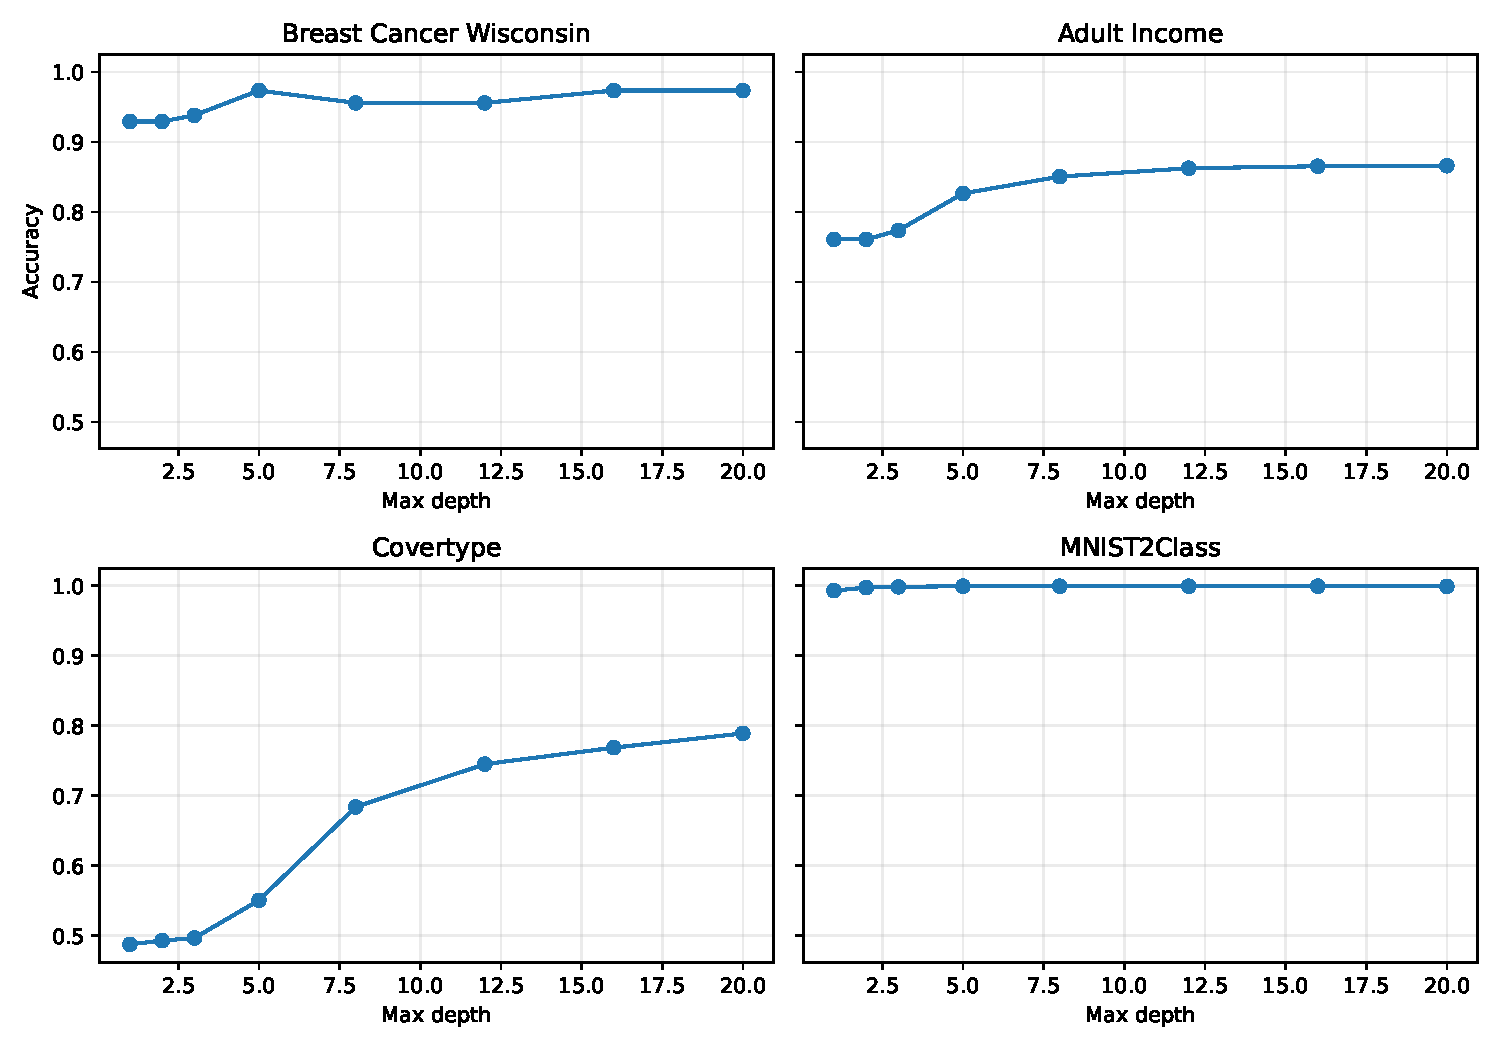
\includegraphics[width=\linewidth]{random_forest_depth.pdf}
\caption{Random Forest test accuracy for depths 1 through 20.}
\label{fig:rfdepth}
\end{figure}

\subsection{Head-to-Head Comparison}
Table~\ref{tab:h2h} gives the complete five-fold summary. Breast Cancer is a
near tie: Random Forest has slightly higher accuracy and macro F1, whereas
AdaBoost has slightly higher AUC. Random Forest leads both custom ensembles
on Adult. On seven-class Covertype, the custom forest strongly exceeds
AdaBoost in accuracy, macro F1, and AUC, although the compiled sklearn
reference remains stronger. Both ensembles are effectively at ceiling on
MNIST2Class.

\begin{table*}[t]
\centering
\scriptsize
\caption{Five-fold cross-validation, mean $\pm$ standard deviation.}
\label{tab:h2h}
\begin{tabular}{llccc}
\toprule
Dataset & Model & Accuracy & Macro F1 & AUC \\
\midrule
Breast & Single Tree & $0.910\pm0.019$ & $0.904\pm0.020$ & $0.905\pm0.023$ \\
Breast & AdaBoost & $0.956\pm0.023$ & $0.952\pm0.025$ & $0.992\pm0.006$ \\
Breast & Random Forest & $0.958\pm0.007$ & $0.955\pm0.007$ & $0.990\pm0.007$ \\
Breast & sklearn RF & $0.953\pm0.020$ & $0.949\pm0.023$ & $0.988\pm0.009$ \\
Adult & Single Tree & $0.814\pm0.002$ & $0.747\pm0.003$ & $0.749\pm0.004$ \\
Adult & AdaBoost & $0.855\pm0.004$ & $0.774\pm0.006$ & $0.907\pm0.004$ \\
Adult & Random Forest & $0.864\pm0.003$ & $0.797\pm0.005$ & $0.917\pm0.003$ \\
Adult & sklearn RF & $0.854\pm0.003$ & $0.788\pm0.004$ & $0.902\pm0.003$ \\
Covertype & Single Tree & $0.811\pm0.004$ & $0.723\pm0.010$ & $0.837\pm0.007$ \\
Covertype & AdaBoost & $0.580\pm0.021$ & $0.320\pm0.025$ & $0.891\pm0.005$ \\
Covertype & Random Forest & $0.813\pm0.004$ & $0.741\pm0.005$ & $0.977\pm0.001$ \\
Covertype & sklearn RF & $0.880\pm0.003$ & $0.814\pm0.007$ & $0.986\pm0.001$ \\
MNIST2 & Single Tree & $0.995\pm0.001$ & $0.995\pm0.001$ & $0.995\pm0.001$ \\
MNIST2 & AdaBoost & $0.999\pm0.000$ & $0.999\pm0.000$ & $1.000\pm0.000$ \\
MNIST2 & Random Forest & $0.999\pm0.000$ & $0.999\pm0.000$ & $1.000\pm0.000$ \\
MNIST2 & sklearn RF & $0.999\pm0.001$ & $0.999\pm0.001$ & $1.000\pm0.000$ \\
\bottomrule
\end{tabular}
\end{table*}

To assess whether the Random Forest vs.\ AdaBoost differences in
Table~\ref{tab:h2h} are more than fold-to-fold noise, we ran a paired
$t$-test (\texttt{scipy.stats.ttest\_rel}) on the five per-fold accuracy
scores of each model for every dataset. Pairing is appropriate here because
both models are evaluated on the identical five folds, so each Random Forest
accuracy is naturally paired with the corresponding AdaBoost accuracy from
the same fold. Because this same test is run
once per dataset, we treat the four accuracy tests as one family and apply
a Holm-Bonferroni correction so the reported significance controls the
family-wise error rate rather than the raw per-test rate; both the raw and
Holm-adjusted $p$-values are written to
\texttt{data/results/head\_to\_head\_significance.csv}. The near tie on
Breast Cancer is not significant either way ($p=0.86$, Holm-adjusted
$p=0.86$), nor is the gap on MNIST2Class ($p=0.14$, Holm-adjusted
$p=0.29$), consistent with both models already sitting near the accuracy
ceiling on those datasets. Random Forest's advantage remains statistically
significant after correction on Adult Income ($p\approx1\times10^{-4}$,
Holm-adjusted $p\approx4\times10^{-4}$) and on Covertype
($p\approx4\times10^{-5}$, Holm-adjusted $p\approx2\times10^{-4}$). Although the paired $t$-test compares the two models on the same folds,
the fold-wise differences are not fully independent because the training
sets in $k$-fold cross-validation overlap substantially.
Consequently, the nominal $p$-values may be somewhat optimistic.
The reported significance tests should therefore be interpreted as
exploratory rather than confirmatory, and are presented alongside,
rather than instead of, the effect sizes reported in
Table~\ref{tab:h2h}.

\subsection{Noise Robustness}
Figure~\ref{fig:noise} evaluates untouched test folds after corrupting only
training labels. At 20\% corruption, Random Forest exceeds AdaBoost on every
dataset (Table~\ref{tab:noise}). The largest separation is Covertype,
0.801 versus 0.678, consistent with boosting's tendency to increase the
influence of mislabeled examples. MNIST2Class remains unusually separable,
but the forest still retains a one-point advantage.

\begin{figure}[t]
\centering
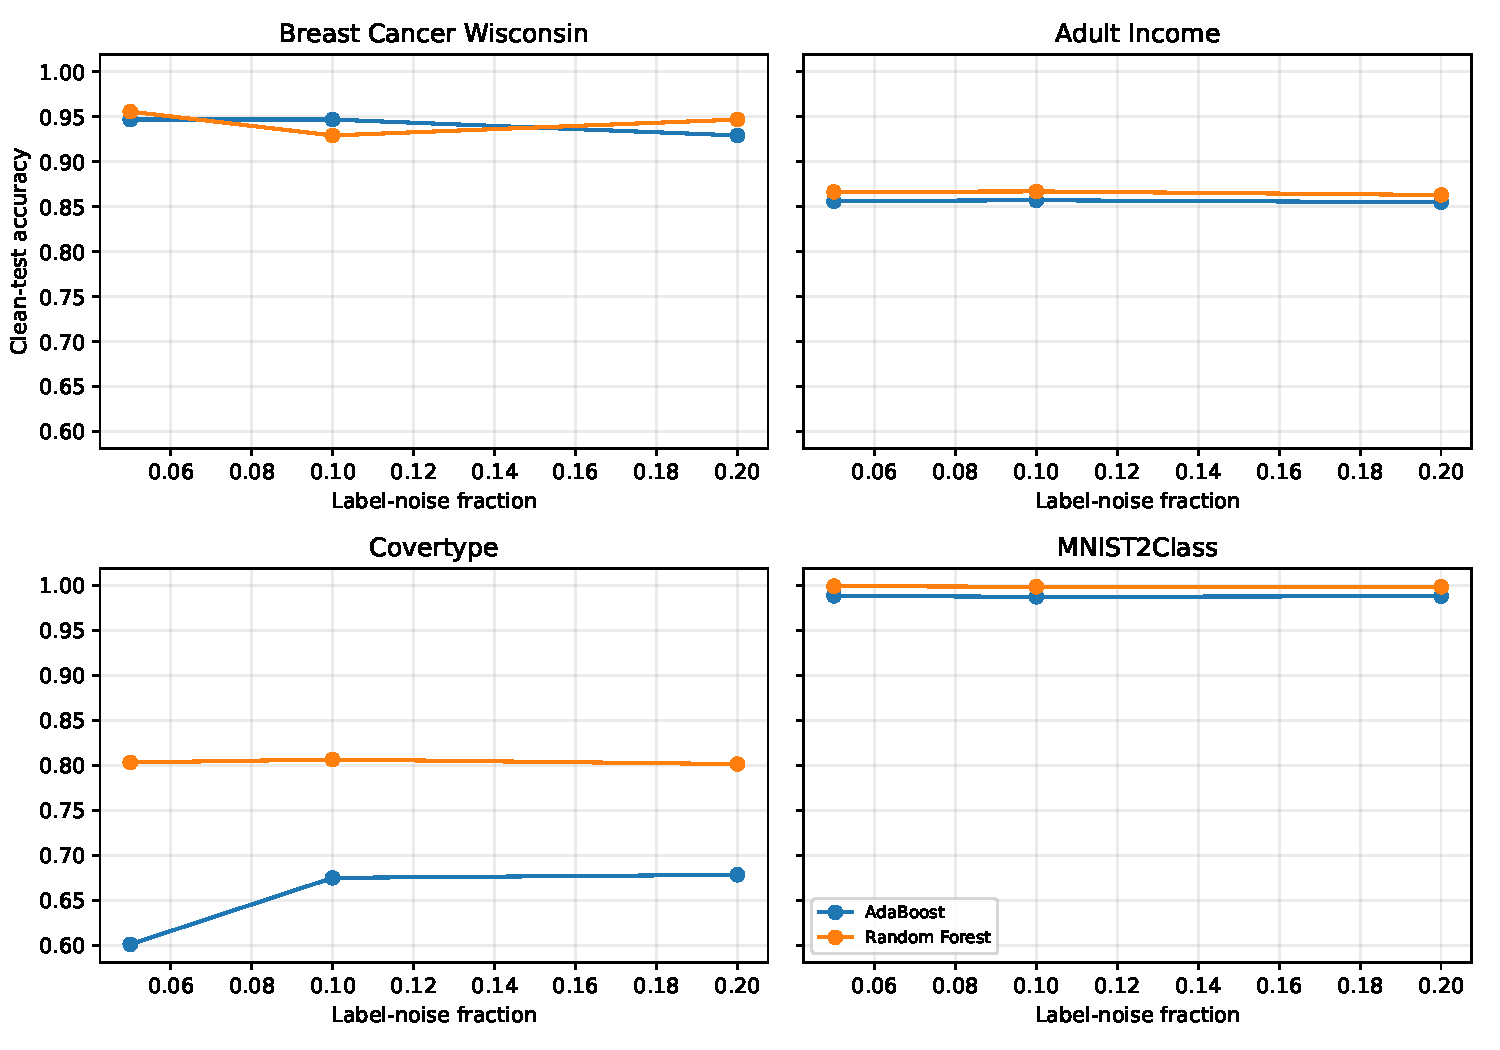
\includegraphics[width=\linewidth]{noise_robustness.pdf}
\caption{Clean-test accuracy after training-label corruption.}
\label{fig:noise}
\end{figure}

\begin{table}[t]
\centering
\caption{Accuracy at 20\% training-label corruption.}
\label{tab:noise}
\begin{tabular}{lcc}
\toprule
Dataset & AdaBoost & Random Forest \\
\midrule
Breast Cancer & 0.929 & 0.947 \\
Adult Income & 0.855 & 0.863 \\
Covertype & 0.678 & 0.801 \\
MNIST2Class & 0.988 & 0.999 \\
\bottomrule
\end{tabular}
\end{table}

\subsection{Real-Data Bias--Variance}
The 100-bootstrap study uses the stratified Breast Cancer 80/20 split, draws
each bootstrap from the fixed training partition, and evaluates every
replicate on the unchanged clean test partition. Table~\ref{tab:bv} shows
that AdaBoost has the lowest expected 0--1 loss (0.0377) and variance
(0.0127) in this setting. Random Forest is second at 0.0473 loss. This
dataset-specific result complements the noise experiment: clean medical data
favors sequential correction, while injected label corruption favors the
forest.

\begin{table}[t]
\centering
\caption{Breast Cancer bias--variance decomposition, 100 bootstraps.}
\label{tab:bv}
\begin{tabular}{lccc}
\toprule
Model & Bias$^2$ & Variance & Loss \\
\midrule
Decision Stump & 0.0973 & 0.0665 & 0.1139 \\
Single Tree & 0.0265 & 0.0542 & 0.0752 \\
AdaBoost & 0.0354 & 0.0127 & 0.0377 \\
Random Forest & 0.0265 & 0.0210 & 0.0473 \\
\bottomrule
\end{tabular}
\end{table}

\begin{figure}[t]
\centering
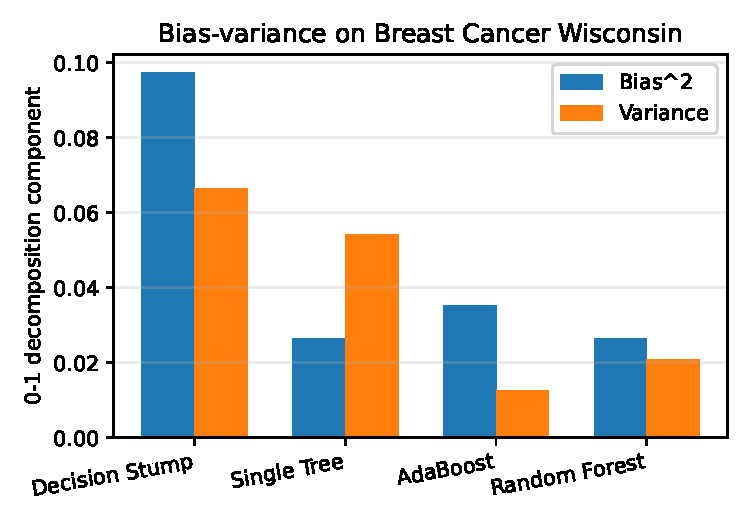
\includegraphics[width=\linewidth]{bias_variance.pdf}
\caption{Real Breast Cancer bias and variance components.}
\label{fig:bv}
\end{figure}

\subsection{Unsupervised Analysis and Bonuses}
Table~\ref{tab:unsup} summarizes complete-data geometry. MNIST2Class needs
150 components for 90\% variance, yet its two digit classes align extremely
well with the nonlinear density/centroid partitions in the first two PCs
(K-Means ARI 0.948; DBSCAN ARI 0.921). Adult and Covertype show much weaker
cluster--label agreement. This warns against treating unsupervised clusters
as class predictions even when supervised accuracy is high.

\begin{table}[t]
\centering
\caption{Full-data PCA and clustering summary.}
\label{tab:unsup}
\begin{tabular}{lcccc}
\toprule
Dataset & PCs$_{90}$ & Best $k$ & KM ARI & DB ARI \\
\midrule
Breast Cancer & 7 & 2 & 0.659 & 0.450 \\
Adult Income & 22 & 3 & 0.132 & 0.063 \\
Covertype & 39 & 4 & 0.091 & 0.133 \\
MNIST2Class & 150 & 2 & 0.948 & 0.921 \\
\bottomrule
\end{tabular}
\end{table}

\begin{figure}[t]
\centering
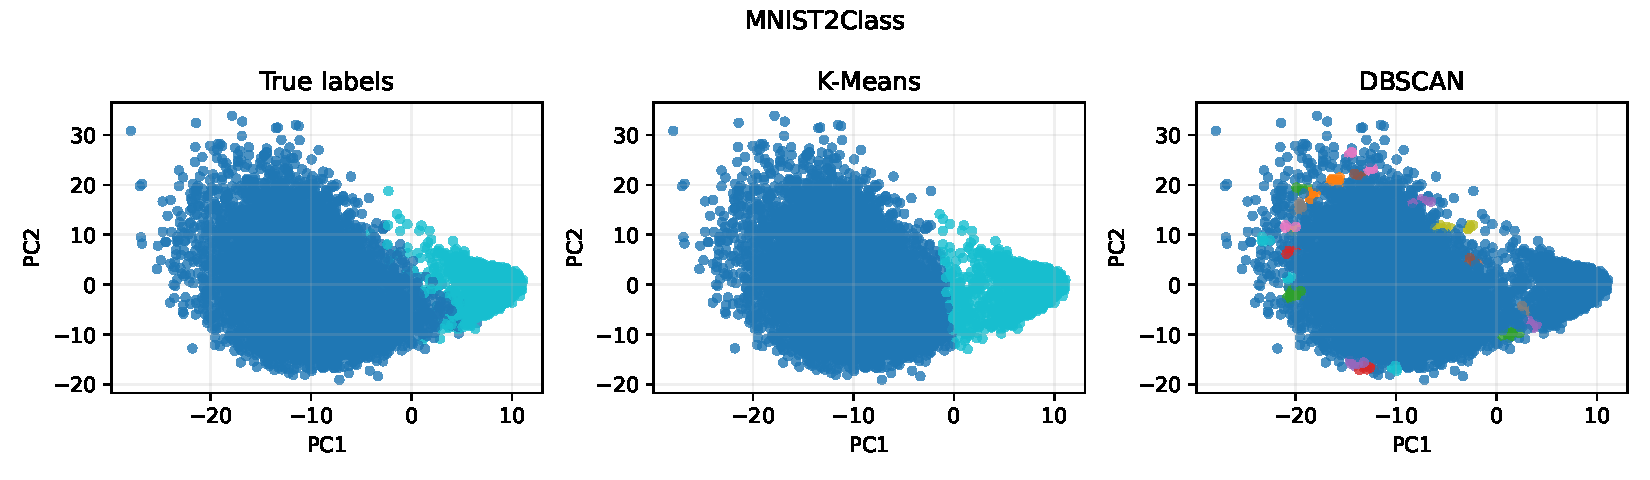
\includegraphics[width=\linewidth]{mnist2class_pca_clusters.pdf}
\caption{Full MNIST2Class PCA projection and cluster assignments.}
\label{fig:pca}
\end{figure}

The full-data t-SNE bonus also uses all 14,780 MNIST2Class rows. On Breast
Cancer, AdaBoost exceeds the optional Gradient Boosting implementation:
accuracy/AUC are 0.973/0.986 versus 0.920/0.964. These bonus results are
reported separately and do not alter the required head-to-head comparison.

\section{Discussion}
The evidence supports a conditional answer rather than a universal winner.
For clean Breast Cancer, the ensembles are nearly tied in cross-validation
and AdaBoost has the stronger bootstrap loss/variance result. On Adult,
Random Forest wins all three custom-model metrics. On Covertype, full-tree
bagging handles seven-class interactions much better than weighted stumps,
and macro F1 exposes AdaBoost's weak minority-class behavior despite its
reasonable one-vs-rest AUC. On MNIST2Class, both approaches are nearly
perfect because zeros and ones are highly separable even though the raw
feature space is large.

Label quality changes the choice. Random Forest wins every 20\%-noise row,
with the largest gain on Covertype. AdaBoost remains attractive when weak
learners identify reliable corrections, but its reweighting mechanism can
overemphasize corrupted observations. OOB accuracy is a useful internal
diagnostic, but it reflects the training transformation and therefore cannot
replace the untouched test metrics, especially for oversampled Covertype.

Threats to validity remain. The transparent NumPy tree backend is much slower
than compiled libraries, so runtime is reported for reproducibility rather
than used as an algorithm-quality claim. Covertype is a deterministic
proportional 50,000-row selection, not the entire 581,012-row population.
The bias--variance decomposition is conditional on one fixed real-data
split, not repeated population draws. Oversampling toward 25\% of the
majority is deliberately simple; class-weighted impurity, calibration, or
threshold tuning may improve minority performance. Finally, DBSCAN uses a
data-derived fifth-neighbor scale in 2D PCA space, so its ARI is descriptive
rather than a tuned supervised result.

\section{Validation and Reproducibility}
Correctness is supported by independent checks: the custom tree remains
within two accuracy points of its sklearn reference on every required
dataset; KD-tree radius/k-nearest results and DBSCAN labels match brute force
on random, duplicate, sparse, and dense fixtures; and a separate 50,000-point
2D DBSCAN smoke test is deterministic without allocating an $n\times n$
array. Mixed preprocessing tests cover missing values, train-only fitting,
unseen categories, deterministic transforms, and retention of all Adult rows.

The default command performs a true full recomputation. The tracked canonical
PR5 artifact run used Python 3.13.3, seed 42, and one forest worker. Its recorded
experimental phases totaled 19,141.946 seconds (5:19:01.946): 1.7 minutes for
baselines, 20.3 for AdaBoost scaling, 85.6 for forest scaling, 118.8 for
cross-validation, 82.0 for noise, 1.5 for bias--variance, 9.0 for unsupervised
analysis including full-data t-SNE, and 0.05 for Gradient Boosting. An
independent C06 reproduction used Python 3.12, seed 42, and four forest workers;
its recorded phases totaled 7,943.706 seconds (2:12:23.706), and all eleven
scientific CSV files matched the canonical run byte-for-byte. The pipeline
produced eleven exact-row CSV tables, two provenance JSON files, and exactly
23 figure PDFs. The opt-in \texttt{--reuse-results} path validates names, row
counts, seeds, grids, fingerprints, and figure names and rejects any mismatch.
Raw and interim downloads stay in ignored cache directories.

\begin{table}[t]
\centering
\caption{Optional bonus items included in the package.}
\label{tab:bonus}
\begin{tabular}{ll}
\toprule
Bonus item & Evidence \\
\midrule
Gradient Boosting & \texttt{src/boosting/gradient\_boosting.py} \\
Full-data t-SNE & \texttt{figures/mnist2class\_tsne\_bonus.pdf} \\
SAMME.R path & \texttt{algorithm="SAMME.R"} \\
GitHub Actions CI & \texttt{.github/workflows/ci.yml} \\
Interactive notebook & \texttt{notebooks/exploration.ipynb} \\
\bottomrule
\end{tabular}
\end{table}

For defense, tree owners should explain weighted impurity and positive-gain
splits; boosting owners should derive SAMME and staged predictions; forest
owners should explain bootstrap/OOB voting and feature subsampling; and
unsupervised owners should explain PCA variance, K-Means inertia, KD-tree
pruning, density reachability, and why ARI is not a supervised score.

\section{Conclusion}
The four-dataset migration changes the empirical answer. AdaBoost is
competitive on clean Breast Cancer and nearly perfect on MNIST2Class, but
Random Forest is the more reliable default on mixed-type Adult, seven-class
Covertype, and corrupted labels. This conclusion follows from one
leakage-controlled pipeline over the exact required rows, with full-data
unsupervised analysis, exact spatial indexing, strict provenance, and no
non-authoritative empirical dataset or silent sample reduction.

\section*{Tools and Acknowledgements}
Substantial AI assistance was used to scaffold, implement, and edit the code
and written materials. The team reviewed the generated code, ran tests, and
kept sklearn ensemble/tree classes out of the project implementations.

\clearpage
\begin{thebibliography}{00}
\bibitem{hastie2009elements}
T. Hastie, R. Tibshirani, and J. Friedman, \emph{The Elements of Statistical
Learning}, 2nd ed. Springer, 2009.

\bibitem{quinlan1986induction}
J. R. Quinlan, ``Induction of decision trees,'' \emph{Machine Learning},
vol. 1, no. 1, pp. 81--106, 1986.

\bibitem{freund1997decision}
Y. Freund and R. E. Schapire, ``A decision-theoretic generalization of
on-line learning and an application to boosting,'' \emph{Journal of Computer
and System Sciences}, vol. 55, no. 1, pp. 119--139, 1997.

\bibitem{breiman1996bagging}
L. Breiman, ``Bagging predictors,'' \emph{Machine Learning}, vol. 24, no. 2,
pp. 123--140, 1996.

\bibitem{breiman2001random}
L. Breiman, ``Random forests,'' \emph{Machine Learning}, vol. 45, no. 1,
pp. 5--32, 2001.

\bibitem{pearson1901lines}
K. Pearson, ``On lines and planes of closest fit to systems of points in
space,'' \emph{Philosophical Magazine}, vol. 2, no. 11, pp. 559--572, 1901.

\bibitem{lloyd1982least}
S. P. Lloyd, ``Least squares quantization in PCM,'' \emph{IEEE Transactions
on Information Theory}, vol. 28, no. 2, pp. 129--137, 1982.

\bibitem{ester1996density}
M. Ester, H.-P. Kriegel, J. Sander, and X. Xu, ``A density-based algorithm
for discovering clusters in large spatial databases with noise,'' in
\emph{Proc. 2nd ACM SIGKDD}, 1996, pp. 226--231.

\bibitem{maaten2008visualizing}
L. van der Maaten and G. Hinton, ``Visualizing data using t-SNE,''
\emph{Journal of Machine Learning Research}, vol. 9, pp. 2579--2605, 2008.

\bibitem{friedman2001greedy}
J. H. Friedman, ``Greedy function approximation: A gradient boosting
machine,'' \emph{Annals of Statistics}, vol. 29, no. 5, pp. 1189--1232, 2001.

\bibitem{uciAdult}
B. Becker and R. Kohavi, ``Adult,'' UCI Machine Learning Repository, dataset
2. [Online]. Available: \url{https://archive.ics.uci.edu/dataset/2/adult}

\bibitem{uciCovertype}
J. Blackard, ``Covertype,'' UCI Machine Learning Repository, dataset 31.
[Online]. Available: \url{https://archive.ics.uci.edu/dataset/31/covertype}

\bibitem{openmlMnist}
OpenML, ``mnist\_784, version 1,'' dataset 554. [Online]. Available:
\url{https://www.openml.org/api/v1/json/data/554}
\end{thebibliography}

\end{document}
